\chapter{Quantitative dynamics of histones in the human cell nucleus}
\label{ch:frap}

  %% I decided to have a chapter precis. That is enough decorative
  %% test for the first page of a chapter.
%  \epigraph{Agora desenmerda-te.}{Portuguese ``saying''}

  %% chapter concept: in this chapter goes the whole kill FRAP project. I started
  %% positive that this should work and so should the text. We start by studying
  %% the technique and list the assumptions it requires. We do one experiment and
  %% face some problems. Each problem has its own section that ends in a solution.
  %% When the solution was not done, we could offer one. The last one is the cause
  %% that this is not possible and has no solution. Conclusion lists all problems
  %% and their solutions again.

  %% AF: Think this needs to be an abstract, summarising capter in 250 words
  %% Why would you have anything else than an abstract?

  \chapterprecis{
    To further the understanding of nucleosome structure and positioning
    in DNA, we aim to measure kinetic differences between wild type and
    mutant histones in live cells. Fluorescent Recovery After Photobleaching
    is a technique successfully used before to show the different kinetics and
    populations between different histone types. Using the same approach with
    our most disrupting histone mutant, we test the limits of FRAP when
    faced with extremely slow exchange ratios.
  }

  \section{Introduction}

  \subsection{Chromatin remodelling and nucleosome structure}

    The building block of eukaryotic chromatin structure is the nucleosome, comprising
    \SI{147}{\bp} of DNA wrapped around an octamer of two copies of core histones H2A,
    H2B, H3, and H4. Nucleosomes are arranged in a linear chain separated by DNA linkers, and
    can be further compacted into higher order chromatin structures. But chromatin extends
    well beyond DNA compaction, it is a dynamic complex that controls access to genetic
    information by undergoing reconfiguration of its structure.

    As the basic structural unit of chromatin, intra-nucleosome interactions
    are the lowest possible level of chromatin configuration. Local reconfiguration
    of chromatin can be achieved by changing nucleosome structure or altering
    its composition. Either via post-translational modifications or incorporation
    of histone variants, nucleosomes may gain different DNA sequence preferences
    or recruit other proteins ultimately changing the chromatin structure.

    Alternatively, chaperones and ATP-dependent chromatin remodelling complexes
    act extrinsically in nucleosome position. One of these is the SWI/SNF~complex
    whose deficiency causes growth defects in yeast. While the exact details of
    its mechanism are not yet known, the contenders being twist defect and
    bulge diffusion, this complex destabilizes the interactions between the
    nucleosome and DNA, causing it to shift position in the DNA sequence.

  \subsection{SIN mutants}

    There is a set of mutations able to compensate the loss of the SWI/SNF
    complex. This set is collectively known as SIN mutations, so named because
    they provide SWI/SNF INdependence. A subset of these are single
    amino-acid changes in the histones sequence, thus suggesting a very
    attractive hypothesis that not only are these locations involved in the
    mechanism of SWI/SNF, but are also of major importance in the nucleosome
    structure. Indeed, this hypothesis has been tested \textit{in vitro}
    where SIN mutant nucleosomes display higher thermal mobility.

  \subsection{FRAP}

    Fluorescence Recovery After Photobleaching (FRAP) is an optical technique
    that reveals the dynamics of fluorescently tagged molecules within live cells.
    The tagged molecules inside a small region are irreversibly photobleached by
    action of a high-power focused laser beam and the recovery rate of fluorescence
    is measured. The recovery rate is interpreted as unbleached molecules,
    which were outside of the region at the time of photobleaching, dissociating and
    diffusing into the bleached area, replacing the bleached molecules. It is assumed that the
    the fluorescence recovery reflects the protein natural movement.

    This technique has been extensively used to obtain qualitative and quantitative
    insight on the kinetic properties of proteins. Among these are also
    histone proteins, where FRAP was used to compare exchange ratios and
    soluble pools of different histones types and variants. These results
    show extremely slow recovery rates, with half-lives longer than 8~hours.

    %%FIXME we should probably be more descriptive of Kimura and Cook results

    Continuous development of FRAP has
    led to increasingly complex models that are both more precise and accurate than simple models
    based on inverse exponential decay.
    However, despite their sophistication, these models of recovery require certain important
    assumptions that are difficult to maintain for long experimental observation times:

    \begin{itemize}
      %% FIXME the first one is not really a problem related to long time FRAP
      \item the biological system has reached equilibrium before photobleaching;
      \item total amount of both Fluorescent Protein (FP) fusion protein and its
            binding sites remain constant over the time course of the recovery;
      %% FIXME we should probably group the 2 before into one
      \item distribution of tagged molecule mimics the endogenous protein;
      \item the binding sites are part of a large, relatively immobile complex, at
            least on the time and length scale of the recovery.
    \end{itemize}

  \subsection{Objectives}

    We aim to develop a technique capable of measuring subtle kinetic
    alterations of the nucleosome in live cells for study of the
    structure--function relationship of the nucleosome.
    Starting with the histone SIN mutant H4~R45H, know \textit{in vitro} to
    cause the highest increase in mobility, we can test FRAP for this
    corner-cases while validating \textit{in vivo} the previous results.

    These results lead to more detailed model of the nucleosome, allowing
    to predict effects of extra mutations which can be feed back to this
    technique for testing. A continuous cycle of this approach will then lead
    to continuous refining of the nucleosome model.


  \section{Materials preparation}

  \subsection{Plasmid construction}

    Plasmids for the canonical histones H2B, H3, and H4,
    respectively pBOS--H2B--GFP, pBOS--H3--EYFP.MC--N1, and pBOS--H4--ECFP.M--N1,
    were provided by Prof. Kevin Sullivan from National University of Ireland,
    Galway. The pBOS--H2B--GFP plasmid has been previously published
    \citep{KevinH2BGFP}. DNA sequencing identified the H3 plasmid as
    the HIST1H3B gene, encoding H3.1 from histone cluster 1; the H4 plasmid
    as either HIST1H4J or HIST1H4K; and the H2B plasmid most similar to the
    HIST1H2BJ gene but with two missense mutations, D25G and V118I.

    Plasmid pPAGFP--N1 and mCherry--\textalpha--tubulin was provided by
    Chelly van Vuuren from National University of Ireland, Galway.

    The HeLa cDNA library was a kind gift by Nadine Quinn from National University
    of Ireland, Galway \citep{NadineThesis}.

    Plasmid pMH3.2--614, which includes a mouse replication dependent histone~H3
    gene, including its upstream and downstream regulatory elements \citep{pMH3-plasmid},
    was provided by Prof. Kevin Sullivan from National University of Ireland, Galway.

    \paragraph{H2B--EGFP}
      The two mutations in the original plasmid were corrected by two
      individual PCR mutagenesis. The first fixed V118I with primers
      AFG112 and AFG113, the second fixed D25G with primers AFG114 and
      AFG115.

    \paragraph{H4--ECFP R45H}
      The R45H mutation was inserted into the pBOS--H4--ECFP.M--N1 by
      PCR mutagenesis using the primers AFG124 and AFG125. The codon
      \texttt{CAC} was selected for the histidine amino acid due to its
      higher codon usage in the human genome\citep{codon_usage}.

    \paragraph{pBOS--GFP}
      A pBOS--GFP vector was prepared from pBOS--H2B--GFP by digestion
      with KpnI and BamHI. The band corresponding to the linearised vector
      without the H2B sequence was purified by gel extraction and used in
      ligation with the H2A sequence.

    \paragraph{H2A--EGFP}
      The H2A sequence was amplified from HeLa genomic DNA with primers
      AFG116 and AFG118. This amplified the coding sequence for the
      HIST1H2AB gene since it has the same sequence used in the previous
      \textit{in vitro} studies that we aim to validate \citep{flaus2004sin}.
      The only other sequence encoding the same protein was HIST1H2AE but has
      a lower codon adaptation index and predicted 5' mRNA secondary
      structures more complex.

    \paragraph{H2AX--EGFP and S139 mutants}
      Closing strategy for cloning the H2AX sequence was similar to the
      strategy for cloning H2A but using the primers AFG130 and AFG131.
      Mutations to H2AX S139, an important site that is phosphorylated during
      DNA damage response,
      was performed at the same time of gene amplification since its location
      is close to the sequence 3' end. The primers AFG132, AFG133, and AFG134,
      were used instead of AFG131 for mutations S139A, S139D, and S139E
      respectively. The mutation to alanine blocks, while
      mutation to aspartic and glutamic acid mimic phosphorylation.
      This strategy introduced an accidental frameshift mutation near the
      stop codon which was fixed by PCR mutagenesis using primers AFG400
      and AFG401.

    \paragraph{H2A.Z--EGFP}
      Unlike the H2A and H2AX plasmids which were prepared from genomic DNA,
      the H2A.Z sequence was amplified from an HeLa cDNA library due
      to the existence of introns in the H2AFZ gene. The amplification PCR
      was performed with primers AFG121 and AFG122. Purification of the
      amplicon and ligation to the pBOS vector was identical to the preparation
      of the H2A--GFP plasmid.

    \paragraph{H4--EYFP}
      The plasmids pBOS--H3--EYFP.MC--N1 and pBOS--H4--ECFP.M--N1 were
      digested with the restriction enzymes BamHI and NotI. After agarose
      gel electrophoresis, the EYFP insert and pBOS--H4 vector were purified
      by gel extraction. The two DNA fragments were ligated to construct
      pBOS-H4-EYFP. The same strategy was used to construct the EYFP tagged
      H4~R45H mutant.

    \paragraph{H3--EYFP T45A and T45E}
      Mutations to H3 T45 were inserted into the pBOS--H3--EYFP.MC--N1 by
      PCR mutagenesis. The primers AFG151 and AFG152 were used for the
      T45E mutation, and AFG153 and AFG154 for T45A.

    \paragraph{H2B and H3 PAGFP}
      The PAGFP insert was prepared from pPAGFP--N1 by PCR using the
      primers AFG478 and AFG479, the amplicon purified by agarose gel
      extraction, digested with NotI and BamHI, and finally cleaned by
      PCR purification.
      Both pBOS--H2B--GFP and pBOS--H3--EYFP.MC--N1 plasmids were also
      digested with NotI and BamHI to excise their tags, and the vectors
      purified by agarose gel extraction. The insert was finally ligated
      into the two vectors for pBOS--H2B--PAGFP and pBOS--H3--PAGFP.
      This strategy introduces a Proline to Arginine mutation in the
      linker for the H2B plasmid.
      %% This mutation in the H2B linker (DPPVAT to DPRVAT) was on purpose.
      %% We could have easily avoid it but would cost us one extra primer
      %% and it shouldn't be making a difference.

    \paragraph{pMH2B--GFP and pMH3--EYFP}
      %% I'm actually not sure if Keving gave me the pMH3.2--614 or the
      %% pCA-TAG plasmid. I did not have any plasmid map or sequence, only
      %% the very small Figure 5 of his paper PMID:9024683
      %% I couldn't even use any standard sequencing primer and by the time
      %% we cloned our genes there, we had already decided to kill the project
      %% so we never got to actually try these in human cells.
      Insertion of the H2B--GFP and H3--EYFP coding sequences into the
      pMH3.2--614 plasmid was performed by PCR amplification, bluent-end
      ligation of both vector and inserts due to the absence of restriction
      sites. pMH3.2--614 was amplified with primers AFG417 and AGF418 which
      create a linear sequence that only ignore the H3.2 coding sequence.
      The H2B--GFP coding sequence was generated with primers AFG419 and AFG420.
      Primers for the insert were phosphorylated by T4~PNK prior to the PCR
      since T4~PNK is more efficient on single stranded DNA. pM vector and
      H2B--GFP insert were purified by agarose gel extraction and ligated.
      Strategy for H3--EYFP was equivalent but using primers AFG424 and AFG420.

  \subsection{Cell lines}

    Transfection was always performed by lipofection~(\Sref{methods:lipofection}),
    both for transient and stable cell lines.

    For creation of stable cell lines, cells were trypsinized and split
    1:20 on \SI{10}{\cm} dishes 24~hours after transfection.
    After another 24 hours, Blasticidin-S was added to the medium for
    a final concentration of \SI{3}{\ug\per\ml} as found by performing a
    Blasticidin-S kill-curve (\Sref{sec:methods:kill-curve}).
    Cell growth was followed and medium replaced when appropriate.
    As cell colonies started to be visible by the naked eye, approximately
    3~weeks after plating, these were screened by fluorescence microscopy.
    Positive colonies were aspirated and moved into 24-well plates with
    \SI{1}{\ml} disposable pipette tips, and the thinnest extremity removed.

    \begin{figure}
      \centering
      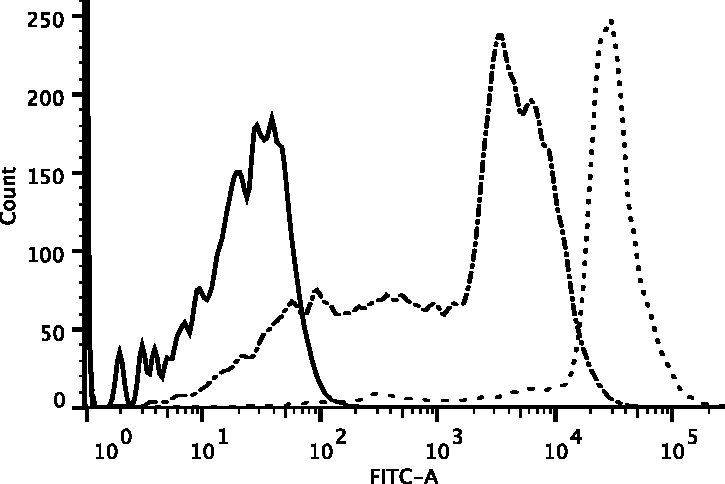
\includegraphics[width=\textwidth]{facs-stable-cell-lines.pdf}
      \captionIntro{FACS sorting of mixed populations}
        {
          The multiple populations with differing intensity values were
          sorted by FACS. The full line represents the intensity profile
          of HeLa wild type cells; the dash-dot line, a mixed population
          of HeLa cells expressing H2B--EGFP; and the dotted line, the
          sorted population.
        }
      \label{fig:methods:facs}
    \end{figure}

    Populations with mixed levels of fluorescent intensity were frequently
    obtained while preparing stable cell lines. In such cases, cells with
    similar intensity of their corresponding fluorophore were FACS
    sorted (\fref{fig:methods:facs}).

    The following stable lines were prepared:

    \begin{itemize}
      \item HeLa H2B--EGFP
      \item HeLa H2B--EGFP D25G V118I
      \item HeLa H3--EYFP
      \item HeLa H3--EYFP T45A
      \item HeLa H3--EYFP T45E
      \item HeLa H4--EYFP
      \item HeLa H4--EYFP R45H
    \end{itemize}

  \subsection{Microscopy}

    Both stable and transiently cell lines were used in imaging. When
    transiently transfected cells were being used, transfection was performed
    approximately 48~hours before imaging.

    Confocal microscopy was performed with a Zeiss LSM510 Meta microscope
    using glass bottom LabTek II chambers. Wide-field fluorescence microscopy
    was performed with an Applied Precision DeltaVision Core system
    using \SI{35}{\mm} glass bottom MatTek dishes.

    In both cases, imaging was performed within an acrylic environmental
    chamber that fully enclosed the stage plate and microscope objectives.
    Temperature and CO$_2$ levels were maintained via separate units connected
    to the environmental chamber.

  \subsection{Computational analysis}

    Software used for image analysis and visualization was described in
    \Sref{sec:methods:software}

    Original source code written in \textsc{Matlab} for a previously
    reported circle FRAP model \citep{mueller2008evidence} was kindly offered
    to us under the GNU General Public License (GPL) version~3 by the
    original authors. A port of this code for the GNU Octave language was
    prepared and made available under the same license.


  \section{Results}

  \subsection{Porting of FRAP analysis}

    For estimation of binding constants from FRAP data, we used a
    previously written model for circle FRAP \citep{mueller2008evidence}.
    The original code was written for the \textsc{Matlab} which we
    ported to GNU Octave.

    While GNU Octave aims to be fully \textsc{Matlab} compatible, certain
    less used features were missing at the time the port was done.
    These could be split into two groups: the functions for nonlinear
    regression \texttt{nlinfit} and \texttt{nlparci} from the Statistics
    Toolbox; and functions for graphical user
    interaction such as \texttt{uigetfile} and \texttt{impoly}.

    Functions for nonlinear regression were required for the model
    fitting and were replaced by \texttt{leasqr}
    from Octave-Forge's optim package. This function performs the
    Levenberg--Marquardt nonlinear least squares algorithm which is the
    same as the documented method for \texttt{nlinfit}.
    Several sample images were analyzed
    by the Octave port and the fitted values were found to be equal to
    the values reported by the authors using the original code.

    Functions for graphical user interaction were mainly required
    for manual selection of Regions Of Interest (ROIs) and options.
    Selection of ROIs was replaced by methods capable of identifying
    them automatically. For setting of different options, a different
    approach was taken and a more typical stand-alone program for batch
    processing, capable of accepting options via command-line was prepared.

    \subsubsection{ROI selection}

      Three different ROIs are required for the used circle FRAP model:
      bleach spot, nucleus region, and background region. The bleach
      spot is required not only to measure the intensity recovery, but
      also to model the photobleach profile since it takes into account
      a non-uniform spatial distribution of the bleach spot. The nucleus
      region to model a finite sized nucleus and consider the fluorescence
      ``destroyed'' during the photobleaching. Finally, a small region
      outside the nucleus is used for background correction.

      Cells expressing GFP tagged histone proteins display a well defined
      nuclei. The high amount of histone protein
      and its specificity for nuclear chromatin, produces a high clear
      signal for the nuclei which contrasted on a dark background (\fref{fig:kill-frap:roi}).

      \begin{figure}
        \centering
        \subbottom[pre-bleach]{
          \includegraphics[width=0.45\textwidth]
          {kill-frap/roi-prebleach.png}
          \label{fig:kill-frap:prebleach}
        }
        \hfill
        \subbottom[post-bleach]{
          \includegraphics[width=0.45\textwidth]
          {kill-frap/roi-postbleach.png}
          \label{fig:kill-frap:postbleach}
        }
        \subbottom[pre-bleach $-$ post-bleach]{
          \includegraphics[width=0.45\textwidth]
          {kill-frap/roi-subtracted.png}
          \label{fig:kill-frap:subtracted}
        }
        \hfill
        \subbottom[Identified ROIs]{
          \includegraphics[width=0.45\textwidth]
          {kill-frap/roi-selected.png}
          \label{fig:kill-frap:selected}
        }
        \captionIntro{Automatic selection of ROIs for FRAP}
          {
            HeLa stable cell line expressing the H4~R45H mutant tagged with YFP,
            are imaged every \SI{30}{\ms} in a confocal microscope. A circular
            shape is used for photobleaching after 100~frames.
            \subcaptionref{fig:kill-frap:prebleach} averaging of 50~pre-bleach
            images removes most of the noise, allowing for a better refined
            ROI;
            \subcaptionref{fig:kill-frap:postbleach} average of
            5 post-bleach images;
            \subcaptionref{fig:kill-frap:subtracted} subtraction of the
            post-bleach to the pre-bleach image, gives a clear indication
            of the bleach spot, as well as faint signal for the nuclear
            region due to unintentional photobleaching;
            \subcaptionref{fig:kill-frap:prebleach} perimeter of the
            automatically identified ROIs superimposed on the pre-bleach
            image: cell nuclei, bleach spot, and background region.
          }
        \label{fig:kill-frap:roi}
      \end{figure}

      Subtraction of the post-bleach (\fref{fig:kill-frap:postbleach}) to
      the pre-bleach (\fref{fig:kill-frap:prebleach}) images displays
      a clear circular shape in a black background corresponding to
      the location of the bleach spot (\fref{fig:kill-frap:subtracted}).
      The centre for the bleach spot was
      identified by finding the maximum of the convolution matrix between
      the subtracted image and a disk kernel. For a reduced signal to noise
      ratio, several pre and post-bleach images were averaged before the
      operations. While the bleach spot is
      the most visible feature, there is also a faint signal on the nuclear
      region which is caused by unintentional photobleaching as result of
      the imaging.

      A rough border of the cell nuclei could be easily defined by
      Otsu's method for image threshold. Similar to the method used
      for identification of the bleach spot, several pre-bleach images
      were averaged before the threshold for a more refined cell border (\fref{fig:kill-frap:selected}).
      Since multiple nuclei often appeared in a single image,
      the coordinates for the bleach spot are used as reference to select
      the correct nucleus.

      The background region was identified by finding the minimum of
      the convolution matrix between the averaged pre-bleach images and
      a small square of black intensity values.

    \subsubsection{Batch processing}

      \begin{sidewaysfigure}
        \includegraphics[width=\textwidth]{kill-frap/frapinator.png}
        \captionIntro{Frapinator visual log files for batch processing}
          {
            Each FRAP experiment generates a log file with 6 different plots
            displaying the analysed values and the fitting to different models.
            In conjunction with the images in \fref{fig:kill-frap:roi} this
            provides a quick overview of the entire analysis process.
            The top left plot displays the raw intensity
            for the background, bleach spot, and nucleus intensity over the
            duration of the FRAP experiment. This is followed by the normalized
            intensity for the bleach spot which is actually used for the
            fitting. The top right displays the intensity
            profile for the bleach spot, and its fit to a radial profile
            model. The three bottom panels display the data fitted to three
            different models: pure diffusion which has no terms for binding
            constants; full model with a fixed diffusion rate; and full model
            with all the 3 terms.
          }
        \label{fig:kill-frap:frapinator}
      \end{sidewaysfigure}

      After we implemented the automatic identification of ROIs, the
      analysis script was turned into a self-contained % or stand-alone?
      program. Since interaction with the Octave interpreter is no
      longer required, a user does not have to ``program'' and can
      abstract from the language it is written. Options can be set via
      the command-line in a typical Unix style, and
      several images are saved with the results and all intermediate analysis
      in the form of visual logs for post-processing analysis.
      These visual logs include the automatically identified ROIs,
      as well multiple plots displaying the measured
      intensities, profile of the bleach spot, and fitting
      to different models \fref{fig:kill-frap:frapinator}.

      With this changes, human interaction was no longer required
      to perform the short time FRAP that the code was originally
      designed for.
      We have named this program frapinator, and made it available
      for public download under the GPL \footnote{\url{https://github.com/af-lab/frapinator}}.


  \subsection{Tracking of cell nuclei}

    %% We could show this but it would only be to "encher chouricos"
%    \begin{figure}
%      \centering
%      \missingfigure{Our first FRAP experiment}
%      \captionIntro{Long time series of HeLa cells expressing H2B--EGFP.}
%                   {Cells were transfected with pBOS--H2B-EGFP and imaged for 8
%                    hours, with intervals of 20 minutes.}
%      \label{fig:kill-frap:cell-movement}
%    \end{figure}

    Due to the extremely slow kinetics of histone proteins, FRAP
    must be performed over several hours where cell movement is
    an issue. % \fref{fig:kill-frap:cell-movement}.
    We tried different approaches to fix this.

    \subsubsection{Higher cell density}

      Initial attempt to limit movement of cells during FRAP
      was to perform the experiment with cells at higher confluence levels.
      Normal cells display contact inhibition, a cellular growth mechanism
      by which cells enter senescence and reduce motion, when
      surrounded by other cells with no free space for movement.

      \begin{figure}
        %% We are only showing one cell rather than the whole field of
        %% of view because otherwise it's hard to notice the movement of
        %% individual cells. If we do display everything, we cell many
        %% nuclei that seem like their movement is smaller. If we do
        %% show it, we comment that we are unsure whether the movement
        %% is cellular or only nuclear.
        \centering
        \includegraphics[width=\textwidth]{kill-frap/confluent-hela.png}
        \captionIntro{Movement of confluent HeLa cells during FRAP experiment}
          {
            Cells reached confluence before the start of the
            experiment in an attempt to reduce motion. Instead, this caused
            cell nuclei to undergo heavy reshape as the cell apparently
            squeezes in between its neighbours. Half-nuclear FRAP performed in
            a confocal microscope over an interval of 8~hours. Top left panel
            is the pre-bleach image, while the others have a time-interval of
            21~minutes. Cells are a stable line derived from HeLa, expressing
            the H4~R45H mutant tagged with YFP.
          }
        \label{fig:kill-frap:confluent-hela}
      \end{figure}

      Cancerous cell lines usually lose this property. However, the reduced
      space should place some restriction in the movement and indeed, we
      observed some decrease of movement but not a complete immobilization.
      Tracking of the ROIs over time was still required \fref{fig:kill-frap:confluent-hela}.

    \subsubsection{Primary cell lines}

      Since HeLa cells, being a cancerous cell line that had lost
      the mechanism through which contact
      inhibition is activated, we experimented with a primary horse
      fibroblast cell line. Using this cell line we were capable to maintain
      a layer of healthy cells covering a Petri dish for several after
      reaching confluence.
      %% cell growth was halted instead of becoming over-confluent

      Transfection of primary cell lines have typically a much lower
      efficiency rate. In addition, we need to image cells after they
      reached confluence, and entered senescence, but transfection
      methods are more efficient when cells are actively dividing
      and lower expression with each cell division. As a compromise,
      we transfected cells \SI{70}{\percent} and imaged after 3 days.

      \begin{figure}
        \centering
        \includegraphics[width=\textwidth]{kill-frap/confluent-horse.png}
        \captionIntro{Movement of confluent primary cells during FRAP experiment}
          {
            Primary horse fibrolasts display contact inhibition and halt growth
            once they reach confluence. However, this does not stop cell
            motion which can still be seen moving. In addition, when compared
            to the cancer cell line HeLa (\fref{fig:kill-frap:confluent-hela}),
            the horse fibroblasts frequently rotated around the $x$ and $y$
            axis. Circle FRAP was performed in a widefield microscope.
            Top left panel is the pre-bleach image, while the others have a
            time-interval of 15~minutes. Cells were transiently transfected
            and are expressing H2B type1-J tagged with EGFP.
          }
        \label{fig:kill-frap:confluent-horse}
      \end{figure}

      However, even after reaching confluence, we observed movement of
      transfected cells \fref{fig:kill-frap:confluent-horse}. Actually,
      the nature of the observed movement was dramatically different from
      the one observed in HeLa cells. All of the transfected cells displayed
      a helix-like movement around the vector of their movement.
      In contrast, rotation of HeLa nuclei was mostly restricted to the
      $z$ axis.

    \subsubsection{CropReg}

      As an alternative to modify the cells behaviour, we implemented a program
      to perform cell tracking. We named this program CropReg
      after its work flow of consecutive image cropping and image registration.

      Firstly, the nuclei of interest is tracked by template-based matching
      by normalized cross-correlation. The nuclei to track
      is identified on the first frame and is used as template against the
      image on the following frame. For increased performance and robustness,
      instead of performing the operation against the entire next frame, only
      the region surrounding its original position is used. Sequential
      usage of this method created a stack of smaller images centred on
      the nuclei of interest.

      Since this was a missing feature in GNU Octave, it was implemented
      upstream, as the ``coeff'' option for scaling in the
      \texttt{xcorr2} function and released as part of the Octave Forge
      signal package version 1.2.0.

      %% TODO since there's more than one way to actually do the normalization,
      %% it might be a good idea to write down the actual math formula

      Secondly, to correct for rotational movement around the $z$ axis, the
      frames were aligned using rigid body geometric transformation from the
      previously released ImageJ plugin StackReg \citep{stackreg}.

      \begin{figure}
        \centering
        \includegraphics[width=\textwidth]{kill-frap/cropreg.png}
        %% imaging was done every 10 minutes, but we are skipping
        %% every other panel
        \captionIntro{Automatic tracking and alignment of moving cells}
          {
            Using CropReg, we successfully tracked individual cells during
            a time-series microscope experiment. The top left corner of each
            panel displays the tracked and aligned cell. Imaging was performed
            in a widefield microscope. Time interval between panels 20~minutes.
            Cells are a stable line derived from HeLa, expressing H3 tagged
            with YFP.
          }
        \label{fig:kill-frap:cropreg}
      \end{figure}

      Using this methodology, we were able to track individual cell nuclei
      throughout the entire FRAP experiments \fref{fig:kill-frap:cropreg} provided
      that nuclei from different cells did not overlap. This was a rare occurrence.

  \subsection{Chromatin movement}

    While performing the FRAP experiments, we observed some movement
    within the cell nuclei. These could not be accounted for simple rotational
    movement around the $x$ or $y$ axis, and resembled more the movement
    of individual bodies within the nuclei.

    \subsubsection{Selection of \G1{} cells}
      %% There's no chemical equilibrium in S phase

      A possible cause of this chromatin movement comes from changes in
      the cell cycle phase. During the S~phase, the DNA is replicated,
      doubling the content of the chromatin.
      More importantly, this breaks
      a core assumption of FRAP, that the system remains in equilibrium
      during the entire experiment. This does not hold if the DNA, the
      binding sites for our model, duplicate in number.

      If the FRAP experiments can't be performed during S~phase and
      mitosis, we are limited to \G1{} and \G2{}. Considering
      the length of the HeLa cell cycle and the requirements to image
      for a time period of 8~hours, we are further limited to \G1{}.
      In addition, the FRAP experiment must be performed early in
      \G1{}~phase to avoid crossing over to the S~phase.

      %% The only reason this was required was because the LSM 510
      %% that we were using could not make Z stack and time lapse
      %% at the same time.
%      \begin{figure}
%        \centering
%        \missingfigure{Hela cells splitting}
%        \captionIntro{Picking cells at early G$_1$.}
%                     {We imaged cells that were entering mitosis and picked their
%                      daughter cells for the FRAP experiments. Because HeLa cells lift
%                      away from the dish during mitosis, opening the
%                      pinhole and set the Z-center in between the cell dividing plane
%                      and dish bottom was necessary. Ends up nothing being properly in focus but we
%                      can track things fine. Of course, some cells still floated away.}
%        %% TODO explicit parameters
%        \label{fig:kill-frap:picking-early-g1}
%      \end{figure}

      To do this, cells in mitosis were selected and tracked during 4~hours.
      After this time period, we used the daughter cells which we could be
      confident of being in early \G1{}.
      %% we also waited some 2 hours after mitosis since that's when cells
      %% unpack their chromosomes.

      During mitosis, HeLa cells form a sphere slightly above the plane of
      other cells, and keep a weak connection to the growth surface.
      Because of this, they easily detach, which is the basis for the
      mitotic shake-off method, and float away from the field of vision
      which requires a larger number
      of initial selected cells. In addition, to minimize any effect that
      may arise from imaging, it was done at minimal laser power and every
      30~minutes, just enough to allow manual tracking.
      Finally, since our system did not permit simultaneous Z-stack and time
      lapse imaging, and cells in mitosis are in a separate focal plane,
      imaging was performed with the pinhole sized to the max and focused
      in between the two planes. While this
      created very blurred images, it allowed to visualize all cells during
      the entire procedure.

      However, even after selecting cells in this cell cycle, movement within
      the bleach spot could still be observed.

    \subsubsection{Inverse FRAP}

      Due to the non-homogeneous nature of the chromatin, it was difficult
      to assess the total extent of the observed movement. To
      better visualize this, we performed inverse FRAP which allows us
      to track the movement of the bleach spot only.

      For this purpose, we replaced the EGFP tag in our H2B plasmid
      with photoactivatable GFP (PAGFP), a GFP derivative that requires
      activation by a specific wavelength to become fluorescent. This
      allows us to activate a specific spot of the nucleus and visualize
      its movement.

      Since PAGFP cannot be easily detected before photoactivation, cells
      were co-transfected with mCherry--\textalpha--tubulin which localises
      exclusively to the cytoplasm, giving an outline of the nuclear region
      \fref{fig:kill-frap:ifrap}.

      \begin{figure}
        \centering
        \subbottom[pre-activation]{
          \includegraphics[width=0.45\textwidth]
          {kill-frap/ifrap-pre.png}
          \label{fig:kill-frap:ifrap-pre}
        }
        \hfill
        \subbottom[post-activation]{
          \includegraphics[width=0.45\textwidth]
          {kill-frap/ifrap-post.png}
          \label{fig:kill-frap:ifrap-post}
        }
        \subbottom[activated spot over time]{
          \includegraphics[width=\textwidth]
          {kill-frap/ifrap.png}
          \label{fig:kill-frap:ifrap-timeframe}
        }
        \captionIntro{Inverse FRAP experiment showing chromatin movement}
          {
            HeLa cells co-transfected with mCherry--\textalpha--tubulin and
            H2B type1-J tagged with PAGFP.
            \subcaptionref{fig:kill-frap:ifrap-pre} The cell nucleus, target
            for photoactivation, can be easily identified as the ``empty''
            region via the mCherry channel on which would otherwise be an
            invisible feature on the GFP channel;
            \subcaptionref{fig:kill-frap:ifrap-post} spot after activation;
            \subcaptionref{fig:kill-frap:ifrap-timeframe} detail of the
            activated spot every 20~minutes. Rather than a gradual loss of
            fluorescence that maintains the circular shape, the activated spot
            kind of unfolds itself spreading the region of interest.
          }
        \label{fig:kill-frap:ifrap}
      \end{figure}

      Using this FRAP variant, the movement of chromatin was more noticeable.
      Rather than an homogeneous loss of fluorescence, the activated
      spot uncurled itself overtime with individual branches of
      localized PA-GFP appearing in the nuclei (\fref{fig:kill-frap:ifrap}).


  \section{Conclusions: why histone dynamics is not measurable by FRAP}
  
  I have attempted to establish FRAP as a method for measurement of histone variants. Such
  an experiment requires observation over an extremely long time interval, challenging several
  assumptions of a typical FRAP experiment.
  
  Workarounds were found to each of them, without the introduction of more factors or decreasing
  the fidelity of the FRAP technique. Except for one, movement of chromatin --- the binding sites.
  This is not easy to observe on a conventional wide-field microscope, and even on a confocal
  microscope is hard to spot. This makes it very easy to go unnoticed. I have performed an iFRAP
  experiment which makes it easier to detect.
  
  While the chromatin movement will not be a problem when performing FRAP on slow exchanging
  proteins, the other issues I found might.
  
  %% FRAP is not goof for very long time frames. Reference papers where it was used incorrectly?
  %% see Tim's paper
  
  Still, alternative techniques might be used to measure dynamics of histone variants in
  live cells. Namely, single molecule tracking would be an ideal candidate provided access
  to the required equipment\addref[has Davide published already about his ``new microscope''
  to do this?].
  
  \todo[inline]{search more for histone and single molecule tracking and imaging}
  
  Single-molecule imaging of histones for short period of times in live cells
  has recently been reported using super-resolution imaging\addref[nature methods 7(9):717-719,
  2010 and nature methods 8(1):7-9, 2011].
   
  Also, use of PA--GFP has been used to measure dynamics of H4 over \SI{90}{\ms} reporting
  differences between interphase chromatin and mitotic chromosomes\addref[Saera Hihara et al 2012].
  However, the difference between these two phases is the highest and might not be comparable to
  the difference between histones variants\todo{study this. Someone must have measured this}.
  
  %% did not mention if FRAP could have been used with H2A and H2B since these move faster after
  %% all. However, the ones really important on the nucleosome structure seem to be H3 and H4, and are
  %% the ones of more interest for us.


